\documentclass[letterpaper, 12pt]{math}

\usepackage{listings}
\lstset{basicstyle=\ttfamily\footnotesize,breaklines=true}
\usepackage{tikz}

\title{CSCI 251: Concepts of Parallel and Distributed Systems}
\author{Alvin Lin}
\date{September 25th, 2017}

\begin{document}

\maketitle

\section*{Topics}
\begin{itemize}
  \item Message Passing
  \item Distributed Memory
  \item Send/receive
  \item Exercise problem
\end{itemize}

\subsection*{Message Passing}
Every processor has its own memory and the processors may be connected
together. They may be connected via a local area network. Every processing unit
has its own local array. Memory is distributed.
\begin{center}
  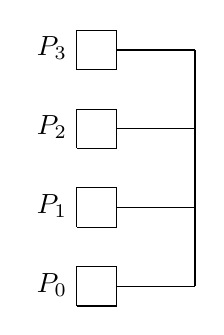
\begin{tikzpicture}
    \foreach \y in {0,...,3} {
      \draw (0,\y) -- (0.5,\y) -- (0.5,\y+0.5) -- (0,\y+0.5) -- (0,\y)
        node[above left] {\( P_\y \)};
      \draw (0.5,\y+0.25) -- (1.5,\y+0.25);
    }
    \draw (1.5,0.25) -- (1.5,3.25);
  \end{tikzpicture}
\end{center}
Processes executing on different processors cannot directly access other
processors, they must request data from other processors. There is
communication and coordination among processes executing in different physical
processing units.
\begin{center}
  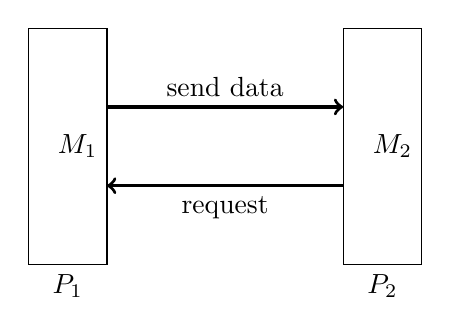
\begin{tikzpicture}
    \draw (0,0) -- node[below] {\( P_1\)} (1,0) -- node[left] {\( M_1 \)} (1,3)
      -- (0,3) -- (0,0);
    \draw (4,0) -- node[below] {\( P_2\)} (5,0) -- node[left] {\( M_2 \)} (5,3)
      -- (4,3) -- (4,0);
    \draw[->,very thick] (4,1) -- (1,1) node[pos=0.5, below] {request};
    \draw[->,very thick] (1,2) -- (4,2) node[pos=0.5, above] {send data};
  \end{tikzpicture}
\end{center}
There are two paradigms for data distribution:
\begin{itemize}
  \item \textbf{Single Program Multiple Data} (SPMD): Identical programs run on
  all the different processors on different data values. In the early days,
  SPMD was called SIMD (Single Instruction Multiple Data).
  \begin{center}
    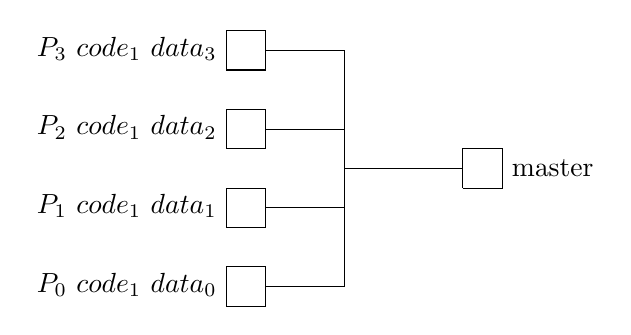
\begin{tikzpicture}
      \foreach \y in {0,...,3} {
        \draw (0,\y) -- (0.5,\y) -- (0.5,\y+0.5) -- (0,\y+0.5) -- (0,\y)
          node[above left] {\( P_\y\ code_1\ data_\y \)};
        \draw (0.5,\y+0.25) -- (1.5,\y+0.25);
      }
      \draw (1.5,0.25) -- (1.5,3.25);
      \draw (1.5,1.75) -- (3,1.75);
      \draw (3,1.5) -- (3.5,1.5) -- node[right] {master} (3.5,2) -- (3,2) --
        (3,1.5);
    \end{tikzpicture}
  \end{center}
  \item \textbf{Multiple Program Multiple Data} (MPMD): Each processor runs a
  separate program. MPMD does not need a master process to divide and handle
  the data.
  \begin{center}
    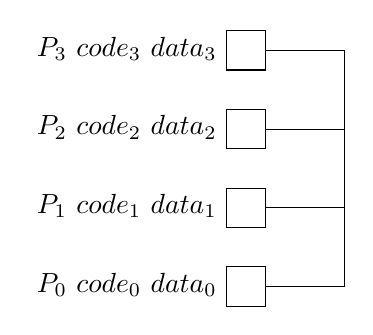
\begin{tikzpicture}
      \foreach \y in {0,...,3} {
        \draw (0,\y) -- (0.5,\y) -- (0.5,\y+0.5) -- (0,\y+0.5) -- (0,\y)
          node[above left] {\( P_\y\ code_\y\ data_\y \)};
        \draw (0.5,\y+0.25) -- (1.5,\y+0.25);
      }
      \draw (1.5,0.25) -- (1.5,3.25);
    \end{tikzpicture}
  \end{center}
\end{itemize}

\subsection*{Send and Receive}
\begin{center}
  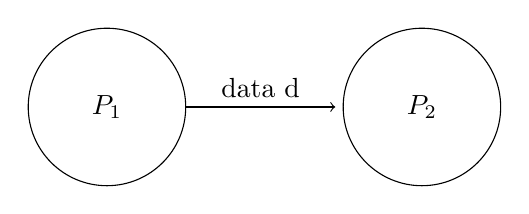
\begin{tikzpicture}
    \draw (0,0) circle (1cm) node {\( P_1 \)};
    \draw[->] (1,0) -- node[pos=0.5,above] {data d} (2.9,0);
    \draw (4,0) circle (1cm) node {\( P_2 \)};
  \end{tikzpicture}
\end{center}
Suppose in the above example, data d is generated by processor \( P_1 \) and
sent to \( P_1 \), which requires the data before it can proceed. There are
four types of data sending which we are concerned with:
\begin{itemize}
  \item \textbf{Blocking and non-buffered}
  \item \textbf{Blocking and buffered}
  \item \textbf{Non-blocking and non-buffered}
  \item \textbf{Non-blocking and buffered}
\end{itemize}
As the name suggests, blocking means that the execution is blocked until the
send and receive is finished. Buffered means that there is a separate memory
segment designated for holding the data when it is created by process \( P_1 \).
\begin{center}
  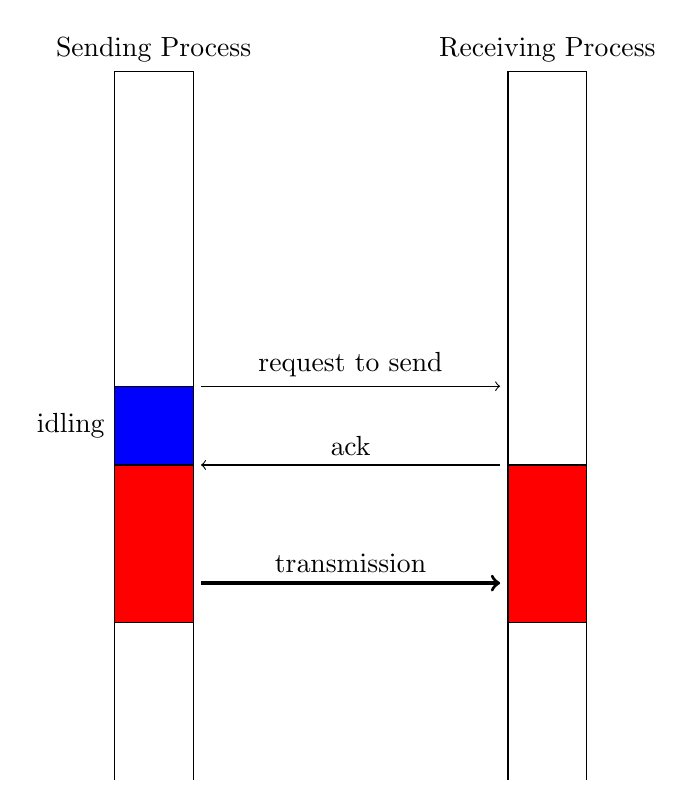
\begin{tikzpicture}
    \draw (0,0) -- node[above] {Sending Process} (1,0) -- (1,-4) -- (0,-4) --
      (0,0);
    \draw[fill=blue] (0,-4) -- (1,-4) -- (1,-5) -- (0,-5) -- node[left] {idling}
      (0,-4);
    \draw (5,0) -- node[above] {Receiving Process} (6,0) -- (6,-5) -- (5,-5) --
      (5,0);
    \draw[->] (1.1,-4) -- node[above] {request to send} (4.9,-4);
    \draw[->] (4.9,-5) -- node[above] {ack} (1.1,-5);
    \draw[fill=red] (0,-5) -- (1,-5) -- (1,-7) -- (0,-7) -- (0,-5);
    \draw[fill=red] (5,-5) -- (6,-5) -- (6,-7) -- (5,-7) -- (5,-5);
    \draw[->,very thick] (1.1,-6.5) -- node[above]{transmission} (4.9,-6.5);
    \draw (0,-9) -- (0,-7) -- (1,-7) -- (1,-9);
    \draw (5,-9) -- (5,-7) -- (6,-7) -- (6,-9);
  \end{tikzpicture}
\end{center}

\subsection*{DMA}
``\textbf{Direct memory access} (DMA) is a feature of computer systems that
allows certain hardware subsystems to access main system memory (Random-access
memory), independent of the central processing unit (CPU). \par
Without DMA, when the CPU is using programmed input/output, it is typically
fully occupied for the entire duration of the read or write operation, and is
thus unavailable to perform other work. With DMA, the CPU first initiates the
transfer, then it does other operations while the transfer is in progress, and
it finally receives an interrupt from the DMA controller when the operation is
done. This feature is useful at any time that the CPU cannot keep up with the
rate of data transfer, or when the CPU needs to perform useful work while
waiting for a relatively slow I/O data transfer. Many hardware systems use
DMA, including disk drive controllers, graphics cards, network cards and
sound cards. DMA is also used for intra-chip data transfer in multi-core
processors. Computers that have DMA channels can transfer data to and from
devices with much less CPU overhead than computers without DMA channels.
Similarly, a processing element inside a multi-core processor can transfer
data to and from its local memory without occupying its processor time,
allowing computation and data transfer to proceed in parallel.''
\textit{-Wikipedia}

\subsection*{Send and Receive Building Blocks}
\begin{lstlisting}
  send(void* sendbuf, int n_elems, int dest);
  receive(void* recvbuff, int n_elems, int source);
\end{lstlisting}
where \texttt{sendbuf} is a pointer to a buffer at the sender's memory that
stores the data to be sent, \texttt{recvbuf} is a pointer to the buffer at
the receiver's memory that stores the received data, \texttt{n\_elems} are
the number the data elements, and \texttt{dest} and \texttt{source} are
identifiers.

\section*{Reminders}
The midterm is on October 11th.
Refer to MyCourses for details on Project 1. \\

\noindent Professor Mohan Kumar: \\
\url{mjkvcs@rit.edu} \\
\url{https://cs.rit.edu/~mjk} \\

\noindent Rahul Dashora (TA): \\
\url{rd5476@mail.rit.edu} \\

\begin{center}
  You can find all my notes at \url{http://omgimanerd.tech/notes}. If you have
  any questions, comments, or concerns, please contact me at
  alvin@omgimanerd.tech
\end{center}

\end{document}
